\chapter{Related Work} \label{cpt-related-work}

The approach we are proposing is an aggregation of a lot of ideas and implementations that have been 
around for quite some time. It is of great interest to explore related work which can provide 
context for use cases and additional techniques. Since our implementation is based on the areas 
of Voxel Redering, Occlusion Culling and Mesh Shading, this chapter will highlight related work 
for each of these topics. 


[@TODO: Check redundancy with technological background]

\section{Voxel Representation} \label{sec-voxel-representation}

\begin{figure}[h]
    \centering
    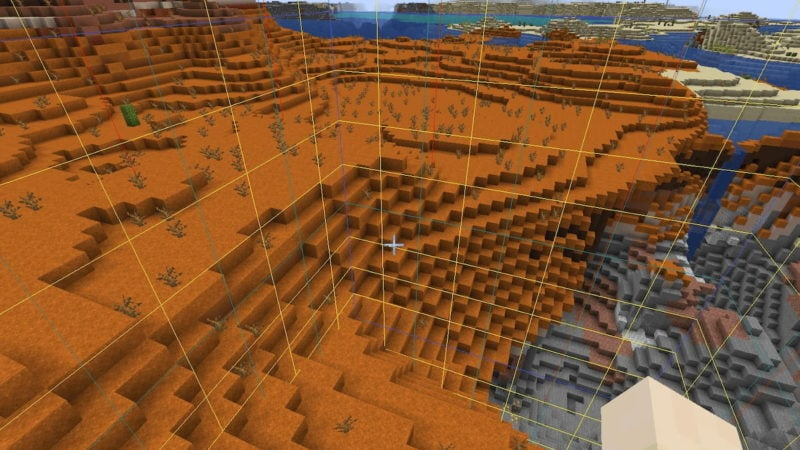
\includegraphics[width=300px]{images/graphics/minecraft-chunks.jpg}
    \caption{A screenshot of minecraft, with a debug visualization of the voxel chunks \cite{Palm2022}.}
    \label{fig:minecraft-chunks}
\end{figure}

\noindent
Voxel Rendering has had huge success in sandbox and highly dynamic games like \emph{Minecraft} (Mojang 
\cite{Mojang2024}, 2011) or \emph{Teardown} (Tuxedo Labs \cite{TuxedoLabs2022}, 2022). Usually these games try 
to preserve some volumetric information for the dynamic environment to be manipulated in real-time. \emph{Minecraft} 
generates a procedural environment based on complex parameters. This way, they can easily generate nearly infinie 
worlds with interesting biomes and landmarks. This huge world is split into chunks of size 16×384×16, to be able to 
stream the world dynamically and allow for quick traversal in any direction, shown in figure \ref{fig:minecraft-chunks}.
Each chunk maintains its own three-dimensional grid, with the voxel data being highly compressed. Non-existing voxels 
are not being stored, and block states, textures and other information is stored in per-chunk buffers or as global 
data in a global buffer. This way, using a texture atlas, up to 256 different texture variants can be easily stored 
per voxel by only one byte \cite{Bergensten2012, MinecraftFandom2021}. \\

\noindent
Many other games have made use of voxel rendering, adapting these principles of data compression and data streaming. 
Most optimizations rely on culling voxels which are not visible, e. g. faces that touch other faces.
Frustum culling and occlusion queries are also part of the optimization process, and partially used in \emph{Minecraft} 
as well (though we cannot finally confirm the existance of frustum culling, or the specific occlusion culling 
algorithm added in version 1.5). Nevertheless, most efforts towards better performance have been on the \ac{CPU} side.
Lately, \ac{GPU}-driven approaches have been implemented by various individual developers. [@TODO: Find specific 
optimizations and sources!]  \\

\noindent
During the past years, ray tracing has become a more common rendering technique, being used for global illumination, 
shadows or ambient occlusion in rasterizer pipelines. Fully ray traced real-time rendering has mostly been available 
for voxel rendering, using common optimization techniques like a \ac{BVH}. Voxel data for ray tracing has been a 
major influence for our approach, since their implicit voxel representation is generally compatible with meshes 
generated directly on the \ac{GPU}. Various efforts have been made to optimize voxel representations for ray traced 
pipelines. Kampe et al. \cite{Kampe2013} propose the use of their \emph{High-Resolution Sparse Voxel \ac{DAG}s}, 
as discussed in chapter \ref{subsec-highres-svo-dags}. This approach is tailored to high voxel resolutions and data that 
might not fit into memory all at once. Their data structure can be easily split up into several sub-trees, which in turn 
can be loaded individually. This approach seems promising for large scenes and use cases, which require the streaming of 
data. 


[@TODO: sources]


\section{Occlusion Culling}





%\section{Minecraft}

%\section{Teardown}

%\section{Assassin's Creed Unity}

%\section{Nanite - Unreal Engine 5}

%\section{Alan Wake / Northlight}


%\section{Octree Occlusion Culling}



- What is it?
- What is interesting about it?
- How does it relate to our work?
- How does it differ from our work?
